\documentclass[a4paper,11pt]{article}
\usepackage[margin=2.5cm]{geometry}
\usepackage{graphicx}
\usepackage{float}
\graphicspath{{figures/}}
\setlength{\parindent}{0pt}
\setlength{\parskip}{0.7em}

\begin{document}

\section*{6.1}
All functions are evaluated at $x\in\{1,\ldots,10\}$ for $i\in\{0.5,1,2\}$.

\textbf{6.1.1: Power functions $F_i(x)=x^i$.}
On linear axes, $x^{0.5}$ grows at a decreasing rate, $x$ grows linearly, and $x^2$ grows at an increasing rate. On logarithmic axes, all three become straight lines because $\log F_i(x)=i\log x$. Their slopes equal the exponents $i$.

\begin{figure}[H]
\centering
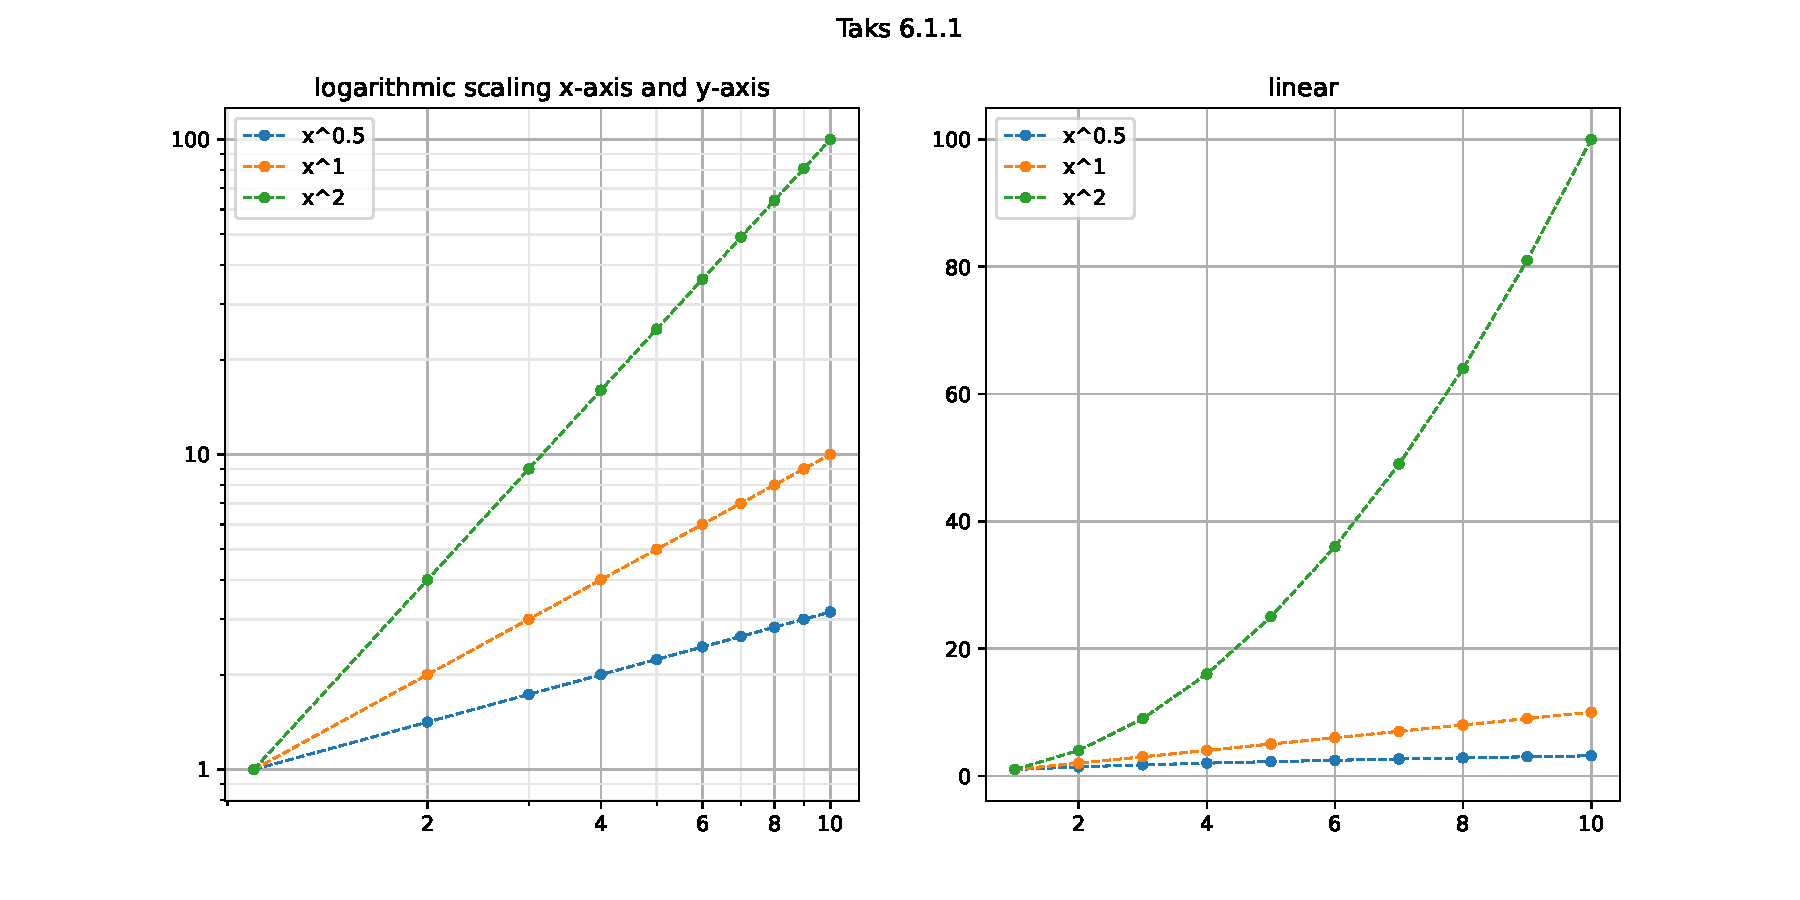
\includegraphics[width=\linewidth,height=0.31\textheight,keepaspectratio]{power-functions.pdf}
\caption{Power functions: logarithmic axes (left) and linear axes (right). The horizontal coordinate is $x$ and the vertical coordinate is $F_i(x)$.}
\end{figure}

\textbf{6.1.2: Exponential functions $F_i(x)=e^{ix}$.}
On linear axes, $e^{2x}$ dominates and compresses the other curves near the horizontal axis. A logarithmic vertical axis makes all three straight lines, since $\ln F_i(x)=ix$, and makes their different growth rates easier to compare. Larger $i$ gives a steeper line.

\begin{figure}[H]
\centering
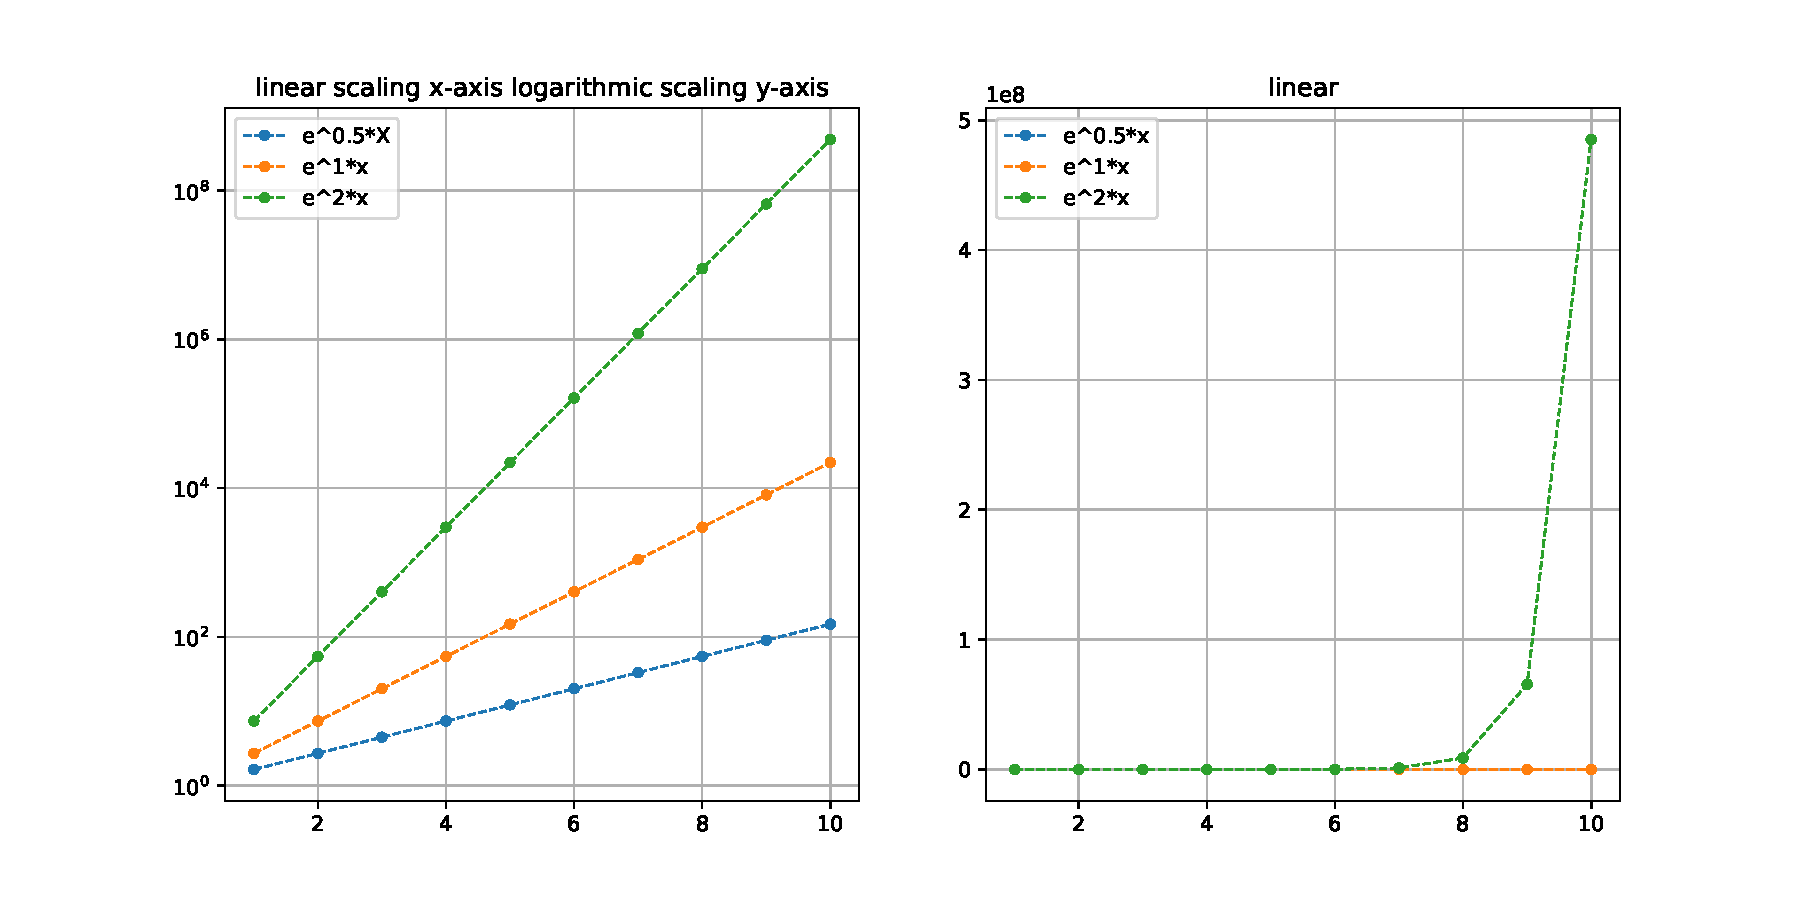
\includegraphics[width=\linewidth,height=0.31\textheight,keepaspectratio]{exponential-functions.pdf}
\caption{Exponential functions: linear horizontal and logarithmic vertical axes (left), and linear axes (right). The coordinates are $x$ and $F_i(x)$.}
\end{figure}

\clearpage
\textbf{6.1.3: Logarithmic functions $F_i(x)=\ln(ix)$.}
On linear axes, all three curves increase at a decreasing rate. With a logarithmic horizontal axis they become parallel straight lines, because $F_i(x)=\ln x+\ln i$. Changing $i$ therefore shifts the curve vertically; adjacent curves differ by $\ln 2$ at every $x$.

\begin{figure}[H]
\centering
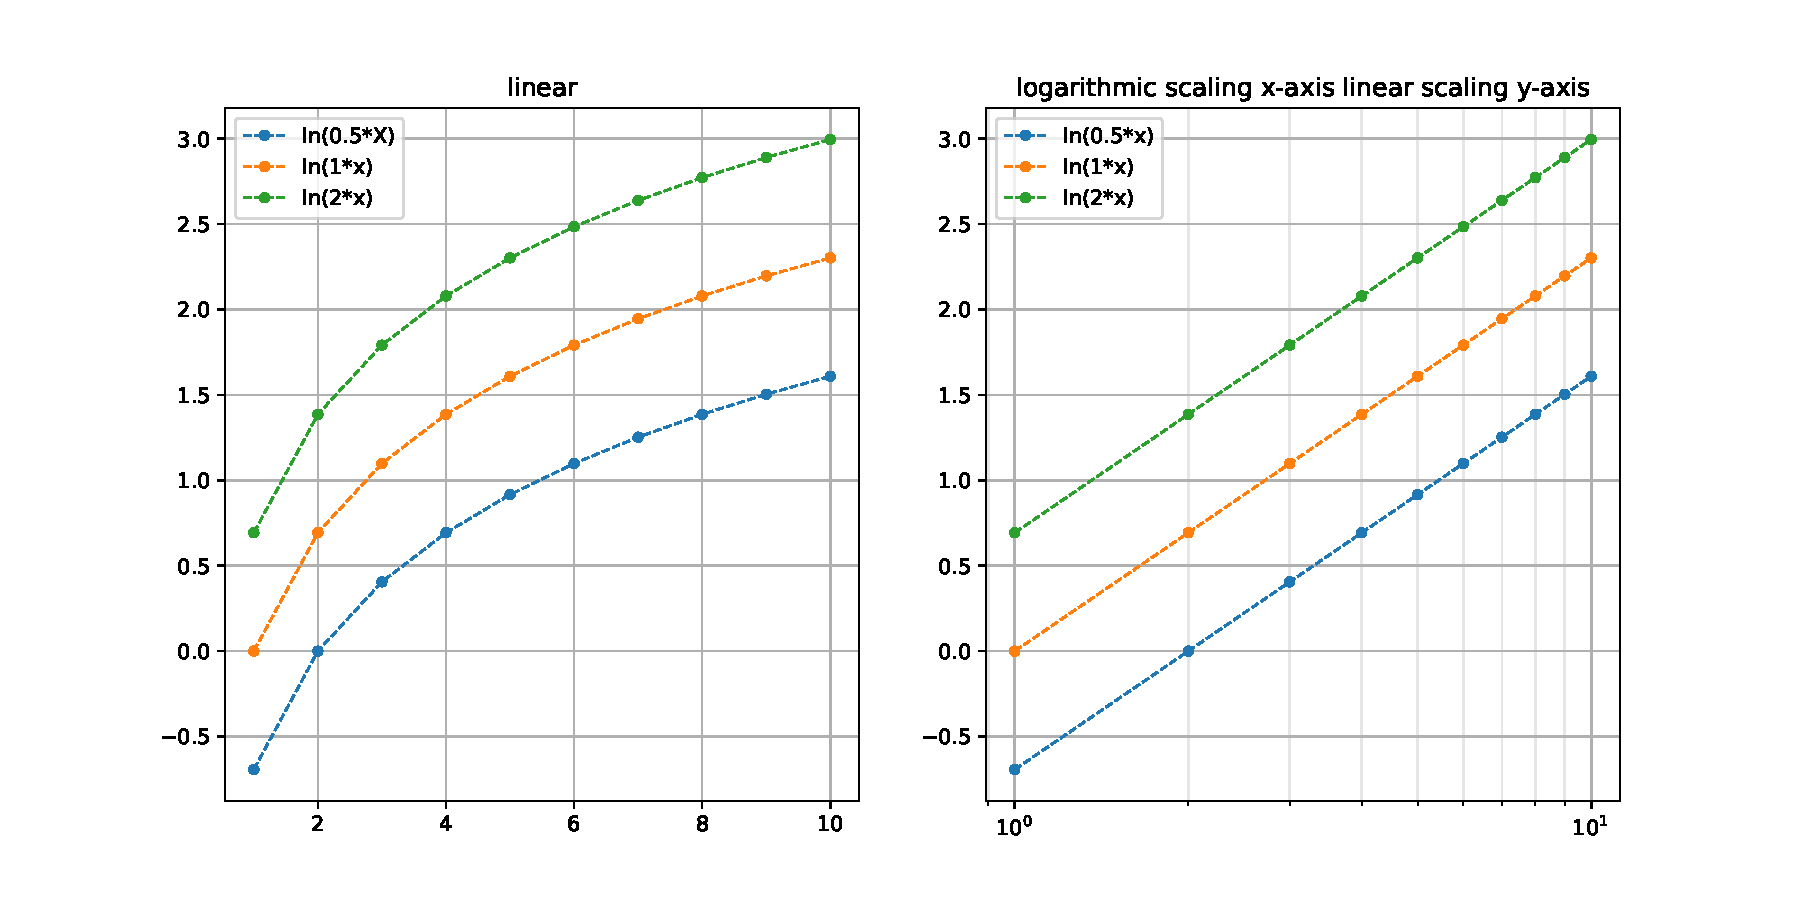
\includegraphics[width=\linewidth,height=0.31\textheight,keepaspectratio]{logarithmic-functions.pdf}
\caption{Logarithmic functions: linear axes (left), and logarithmic horizontal and linear vertical axes (right). The coordinates are $x$ and $F_i(x)$.}
\end{figure}

\clearpage
\section*{6.2}

\textbf{Unemployment over time.}
The unweighted mean unemployment rate across states fluctuates considerably, with peaks in 1975 (8.05\%) and 1982--1983 (about 9.3\%), followed by a decline to 6.93\% in 1986.

\begin{figure}[H]
\centering
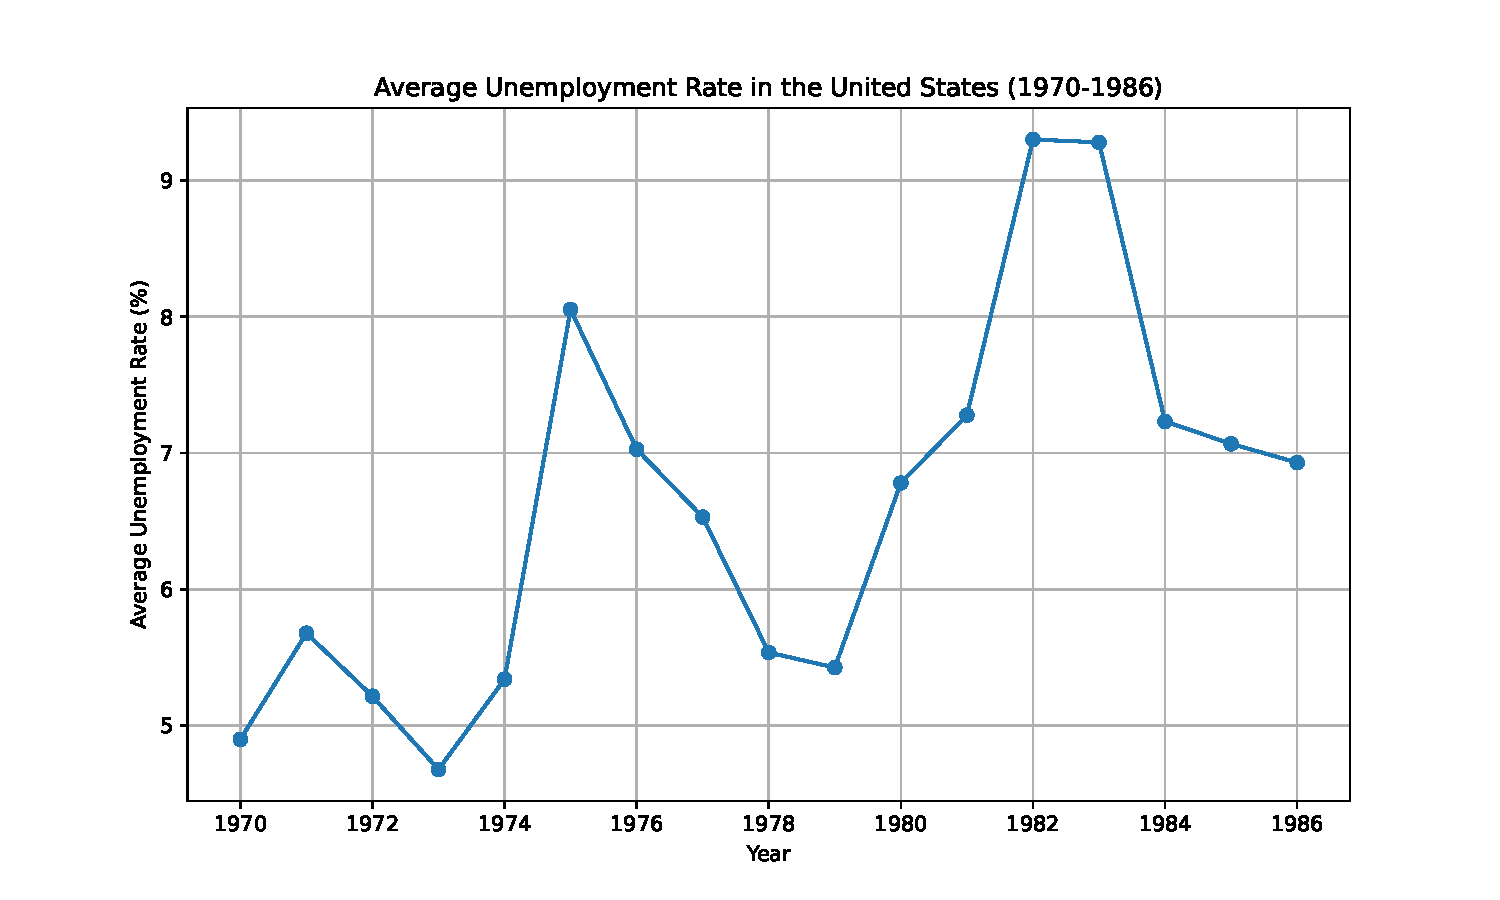
\includegraphics[width=0.9\linewidth,height=0.29\textheight,keepaspectratio]{average-unemployment.pdf}
\caption{Unweighted mean unemployment rate across the 48 states.}
\end{figure}

\textbf{Private capital.}
California, New York, Texas, Illinois, and Pennsylvania have the highest average private capital. California and New York remain clearly ahead, while Texas shows sustained growth.

\begin{figure}[H]
\centering
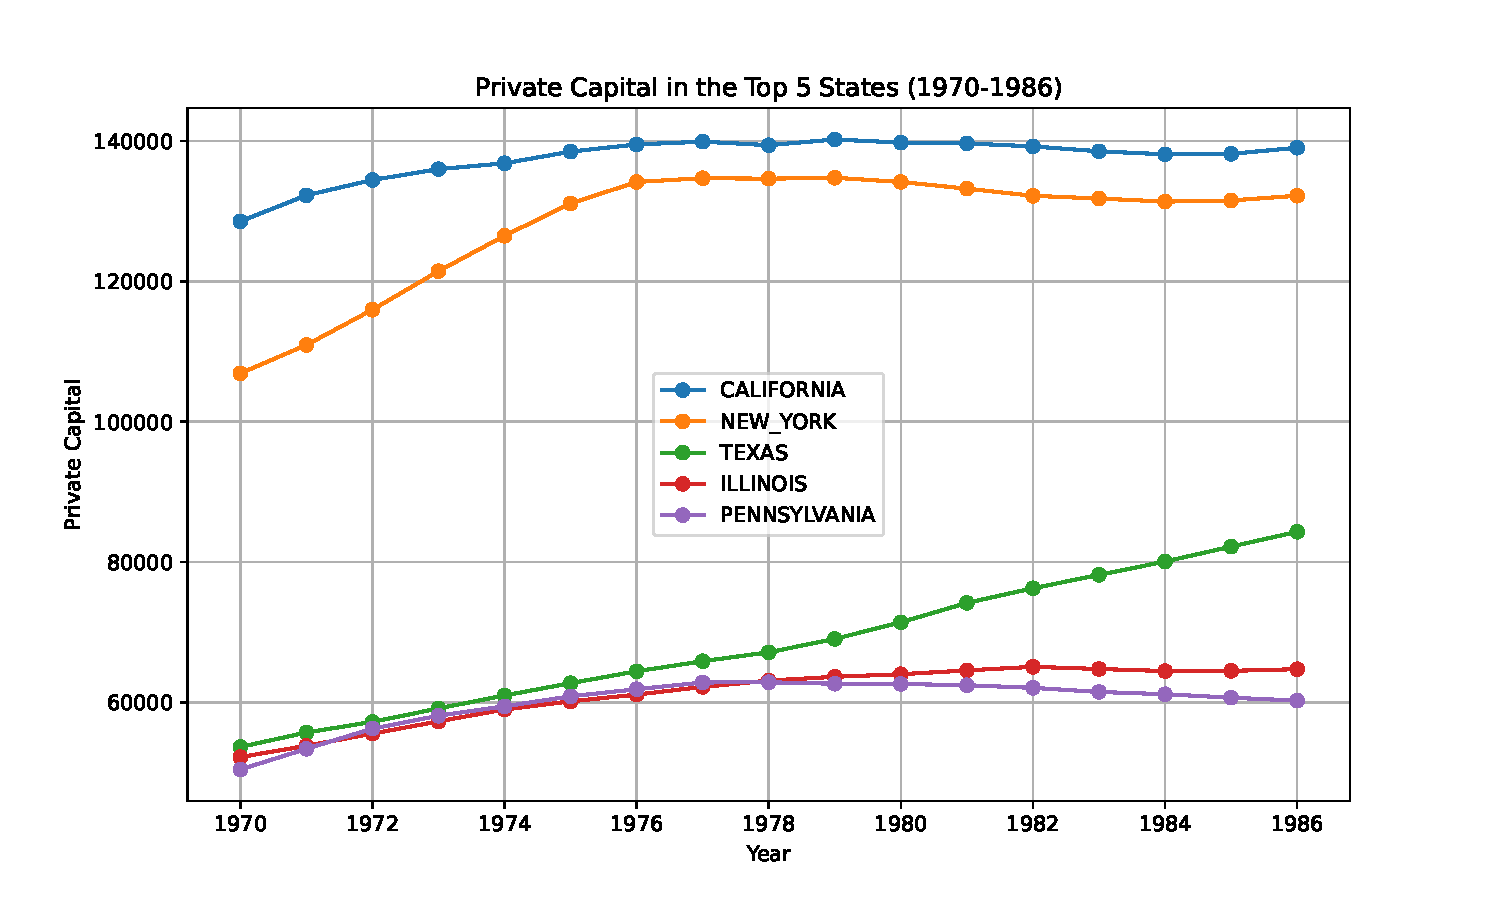
\includegraphics[width=0.9\linewidth,height=0.29\textheight,keepaspectratio]{private-capital.pdf}
\caption{Private capital in the five states with the highest period averages.}
\end{figure}

\clearpage
\textbf{Public capital.}
Average public capital is highest in Texas and lowest in Vermont; both end above their 1970 levels.

\begin{figure}[H]
\centering
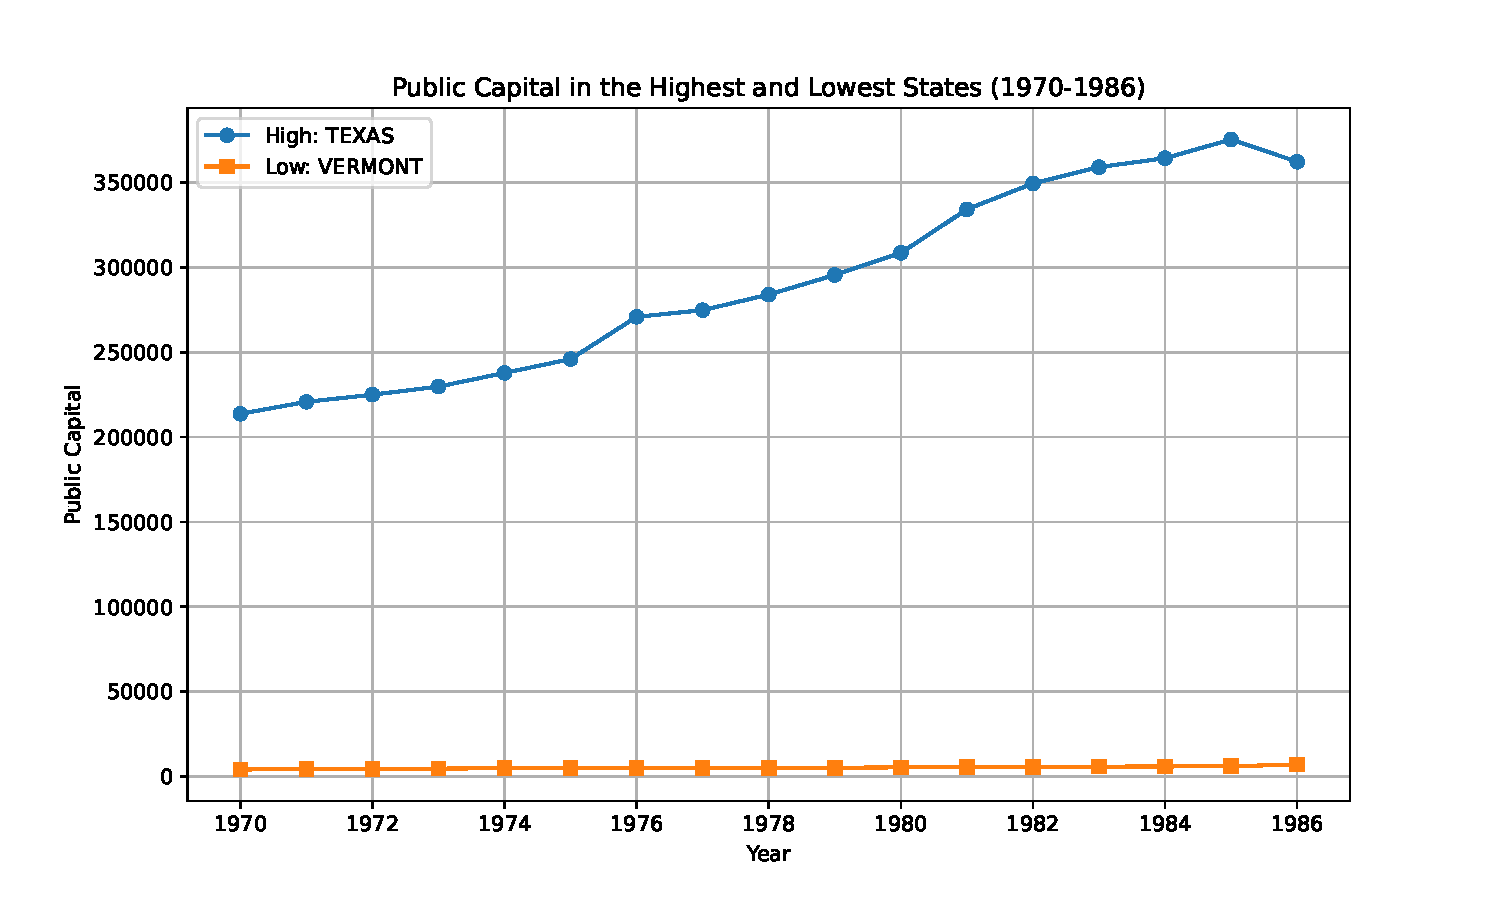
\includegraphics[width=0.9\linewidth,height=0.29\textheight,keepaspectratio]{public-capital.pdf}
\caption{Public capital in the states with the highest and lowest period averages.}
\end{figure}

\textbf{Unemployment boxplots.}
Michigan and West Virginia have the highest mean unemployment rates (9.69\% and 9.27\%). Michigan has the higher median (8.8\% versus 7.5\%), whereas West Virginia has greater variability and a higher maximum (18\% versus 16\%).

\begin{figure}[H]
\centering
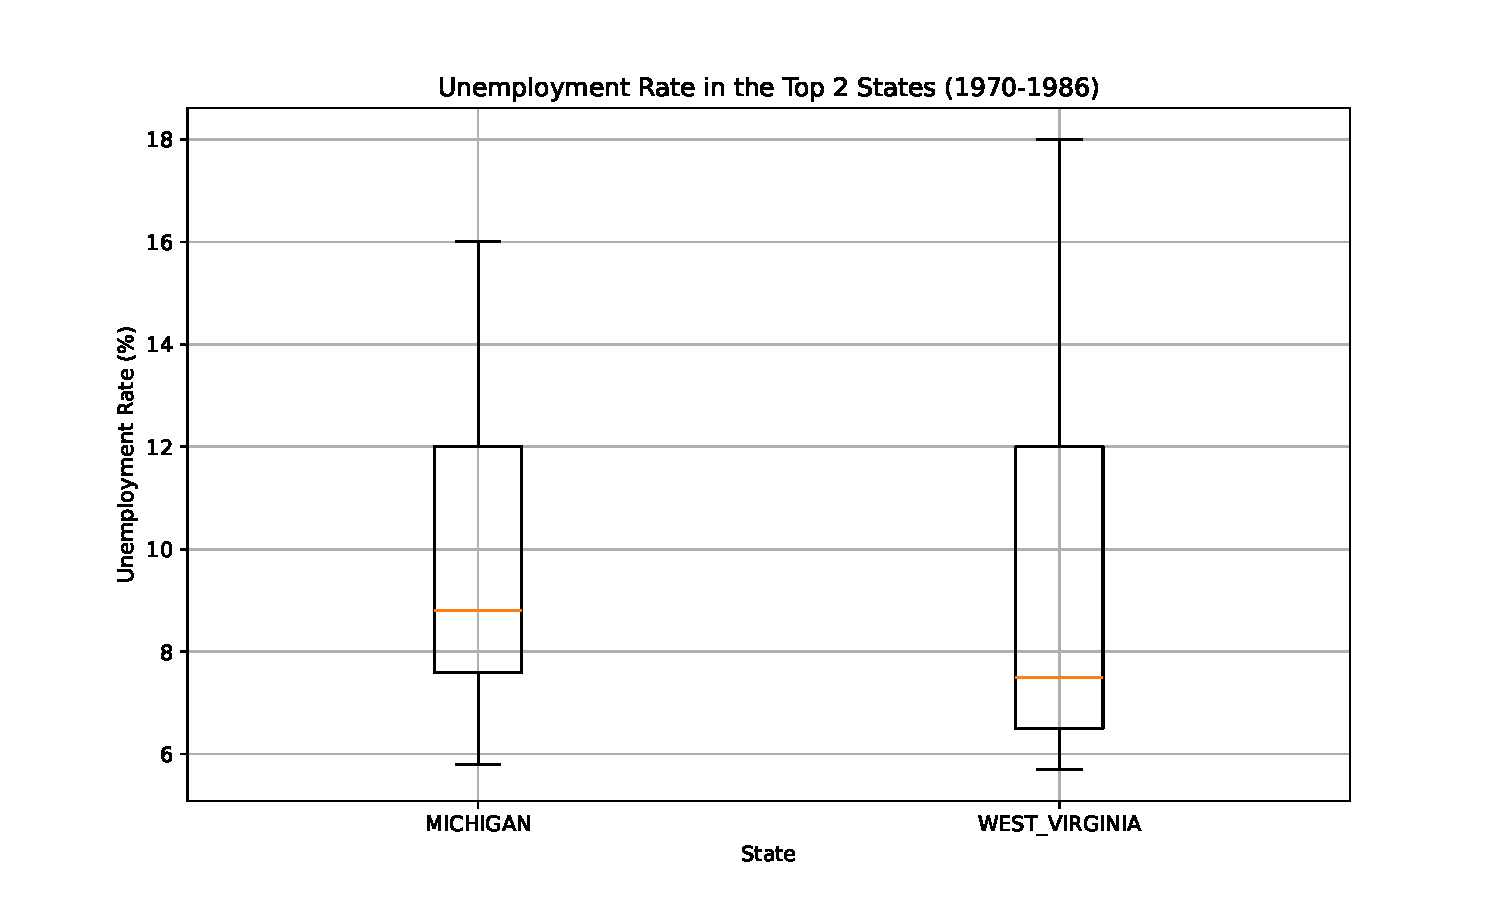
\includegraphics[width=0.9\linewidth,height=0.29\textheight,keepaspectratio]{unemployment-boxplots.pdf}
\caption{Annual unemployment rates in Michigan and West Virginia, 1970--1986.}
\end{figure}

\clearpage

\textbf{Highway and street capital boxplots.}
Vermont and Rhode Island have the lowest mean values. Rhode Island has a slightly higher median and roughly twice the interquartile range, indicating greater variation over time.

\begin{figure}[H]
\centering
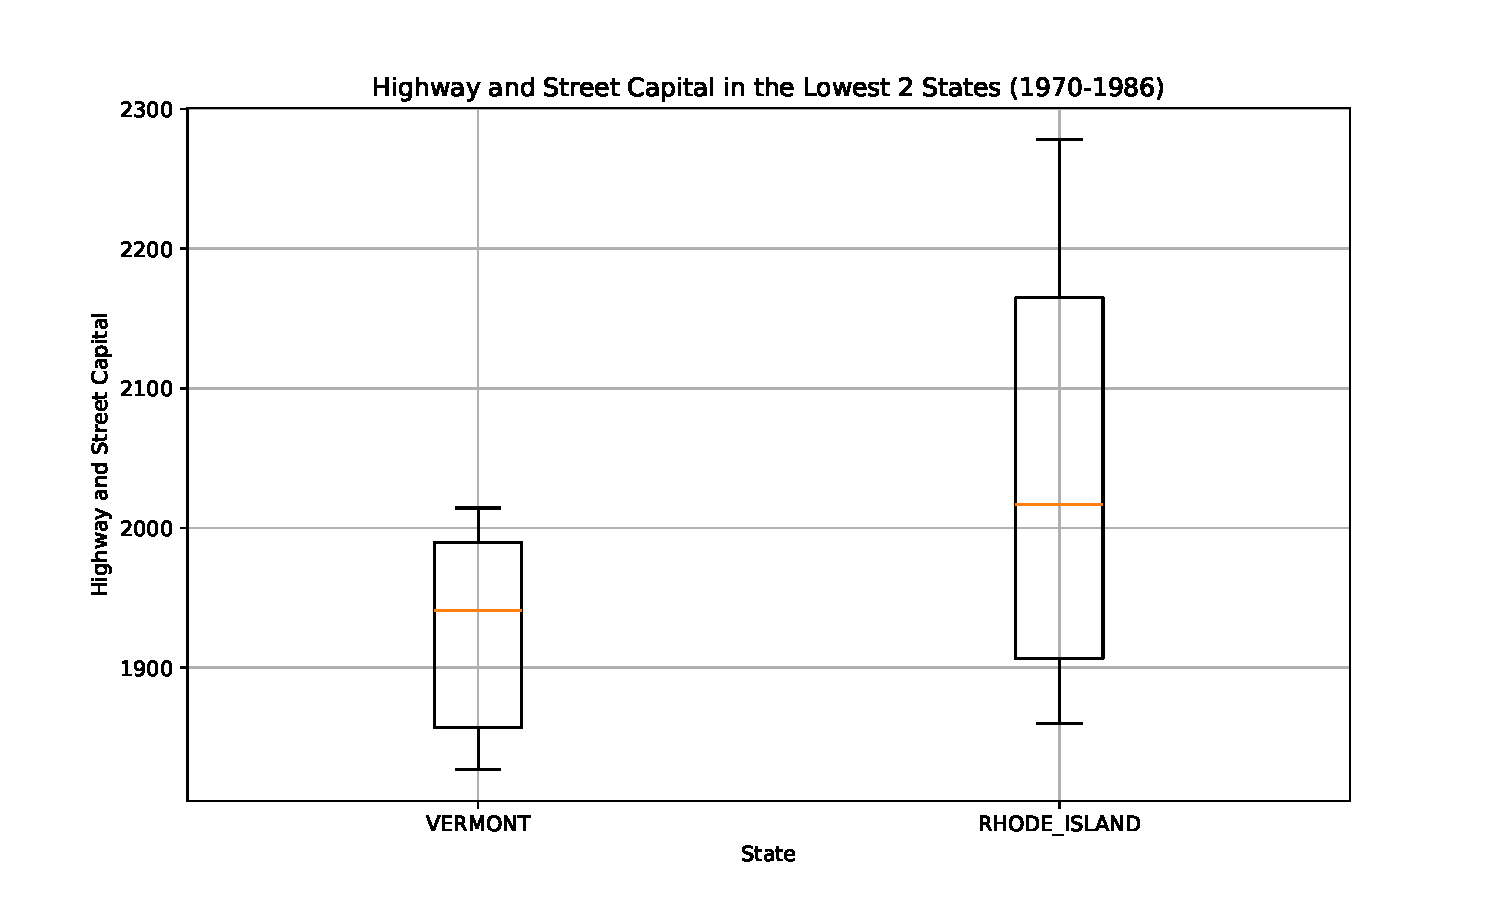
\includegraphics[width=0.9\linewidth,height=0.29\textheight,keepaspectratio]{highway-capital-boxplots.pdf}
\caption{Annual highway and street capital in Vermont and Rhode Island, 1970--1986.}
\end{figure}

\textbf{Employment and unemployment.}
The Pearson correlation between the 17 annual state means is $r \approx 0.505$, indicating a moderate positive association. Employment is an absolute count, whereas unemployment is a share of the labour force, so both can increase when the labour force grows. The correlation of these time series does not establish causation or describe the relationship within individual states.

\begin{figure}[H]
\centering
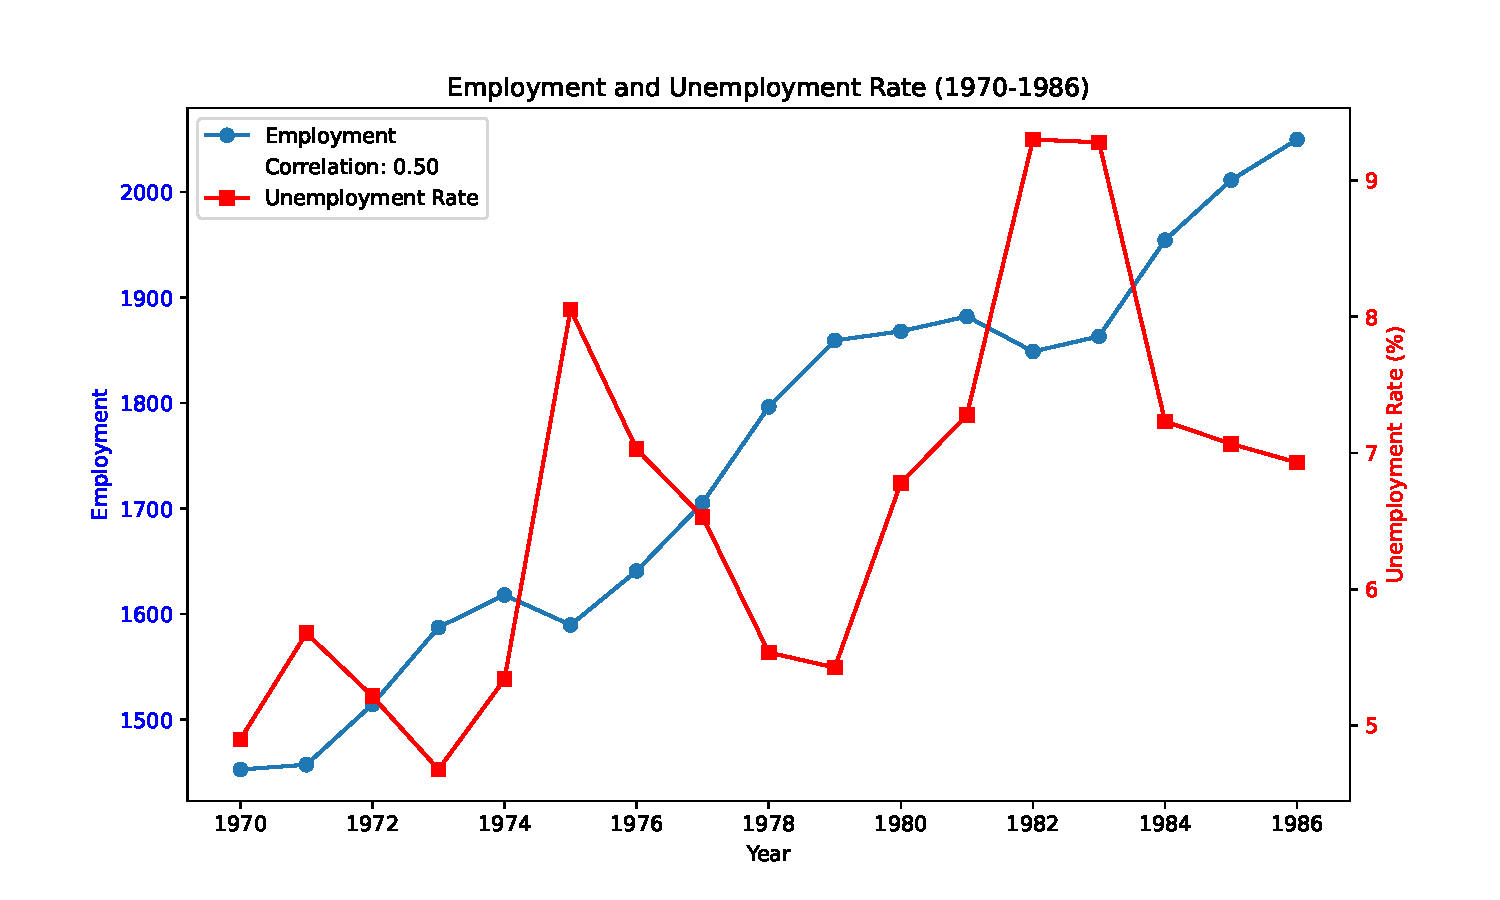
\includegraphics[width=0.9\linewidth,height=0.29\textheight,keepaspectratio]{employment-unemployment.pdf}
\caption{Annual mean employment and unemployment rate, using separate vertical axes.}
\end{figure}

\end{document}
